\documentclass[12pt,a4paper]{article}
\usepackage[utf8]{inputenc}
\usepackage[T1]{fontenc}
\usepackage{amsmath, amssymb, amsthm}
\usepackage{graphicx}
\usepackage{hyperref}
\usepackage{geometry}
\geometry{a4paper, margin=2.5cm}

\title{9. naloga: Spektralne metode za začetne probleme PDE}
\author{Student}
\date{\today}

\begin{document}

\maketitle

\section{Uvod}

V tej nalogi rešujemo enorazsežno difuzijsko enačbo:
\[
\frac{\partial T}{\partial t} = D \frac{\partial^2 T}{\partial x^2}, \quad 0 \leq x \leq L,
\]
z začetnim pogojem:
\[
T(x,0) \propto e^{-\frac{(x - L/2)^2}{\sigma^2}},
\]
in z dvema vrstama robnih pogojev:
\begin{enumerate}
    \item \textbf{Periodični robni pogoji}: $T(0,t) = T(L,t)$
    \item \textbf{Homogeni Dirichletovi robni pogoji}: $T(0,t) = T(L,t) = 0$
\end{enumerate}

Za reševanje uporabljamo dve spektralni metodi:
\begin{itemize}
    \item \textbf{Fourierova metoda} s časovno integracijo po Eulerju
    \item \textbf{Kolokacijska metoda} s kubičnimi B-zlepki in implicitno časovno integracijo
\end{itemize}

\section{Teoretične osnove}

\subsection{Fourierova metoda}

Rešitev razvijemo v Fourierovo vrsto:
\[
T(x,t) = \sum_{k=0}^{N-1} \hat{T}_k(t) e^{-2\pi i f_k x},
\]
kjer je $f_k = k/L$. Po vstavljanju v PDE dobimo:
\[
\frac{\partial \hat{T}_k}{\partial t} = -4\pi^2 D f_k^2 \hat{T}_k.
\]

Za časovno integracijo uporabimo \textbf{Eulerjevo metodo}:
\[
\hat{T}_k(t+h) = \hat{T}_k(t) + h \cdot (-4\pi^2 D f_k^2) \hat{T}_k(t).
\]

Za stabilnost mora veljati:
\[
|1 - 4\pi^2 D f_k^2 h| < 1.
\]

\subsection{Kolokacijska metoda s kubičnimi B-zlepki}

Rešitev aproksimiramo kot:
\[
T(x,t) = \sum_{k=-1}^{N+1} a_k(t) B_k(x),
\]
kjer so $B_k(x)$ kubični B-zlepki. Po vstavljanju v PDE in izvrednotenju v kolokacijskih točkah $x_j$ dobimo sistem ODE:
\[
A \mathbf{a}'(t) = B \mathbf{a}(t),
\]
kjer sta $A$ in $B$ tridiagonalni matriki:
\[
A = \begin{pmatrix}
4 & 1 & & \\
1 & 4 & 1 & \\
& \ddots & \ddots & \ddots \\
& & 1 & 4
\end{pmatrix}, \quad
B = \frac{6D}{\Delta x^2} \begin{pmatrix}
-2 & 1 & & \\
1 & -2 & 1 & \\
& \ddots & \ddots & \ddots \\
& & 1 & -2
\end{pmatrix}.
\]

Za časovno integracijo uporabimo \textbf{implicitno metodo} (Crank–Nicolson):
\[
\left(A - \frac{\Delta t}{2} B\right) \mathbf{a}^{n+1} = \left(A + \frac{\Delta t}{2} B\right) \mathbf{a}^n.
\]

\section{Numerična implementacija}

Implementirali smo obe metodi v Pythonu:

\subsection{Fourierova metoda}

\begin{itemize}
    \item Uporaba FFT za hitro transformacijo
    \item Možnost izbire med periodičnimi in Dirichletovimi robnimi pogoji
    \item Eulerjeva časovna integracija s kontrolo stabilnosti
\end{itemize}

\subsection{Kolokacijska metoda}

\begin{itemize}
    \item Implementacija kubičnih B-zlepkov
    \item Konstrukcija tridiagonalnih matrik $A$ in $B$
    \item Implicitna časovna integracija (Crank-Nicolson) za večjo stabilnost
    \item Reševanje linearnih sistemov v vsakem časovnem koraku
\end{itemize}

\section{Rezultati}

\subsection{Primerjava metod}

\begin{figure}[h]
    \centering
    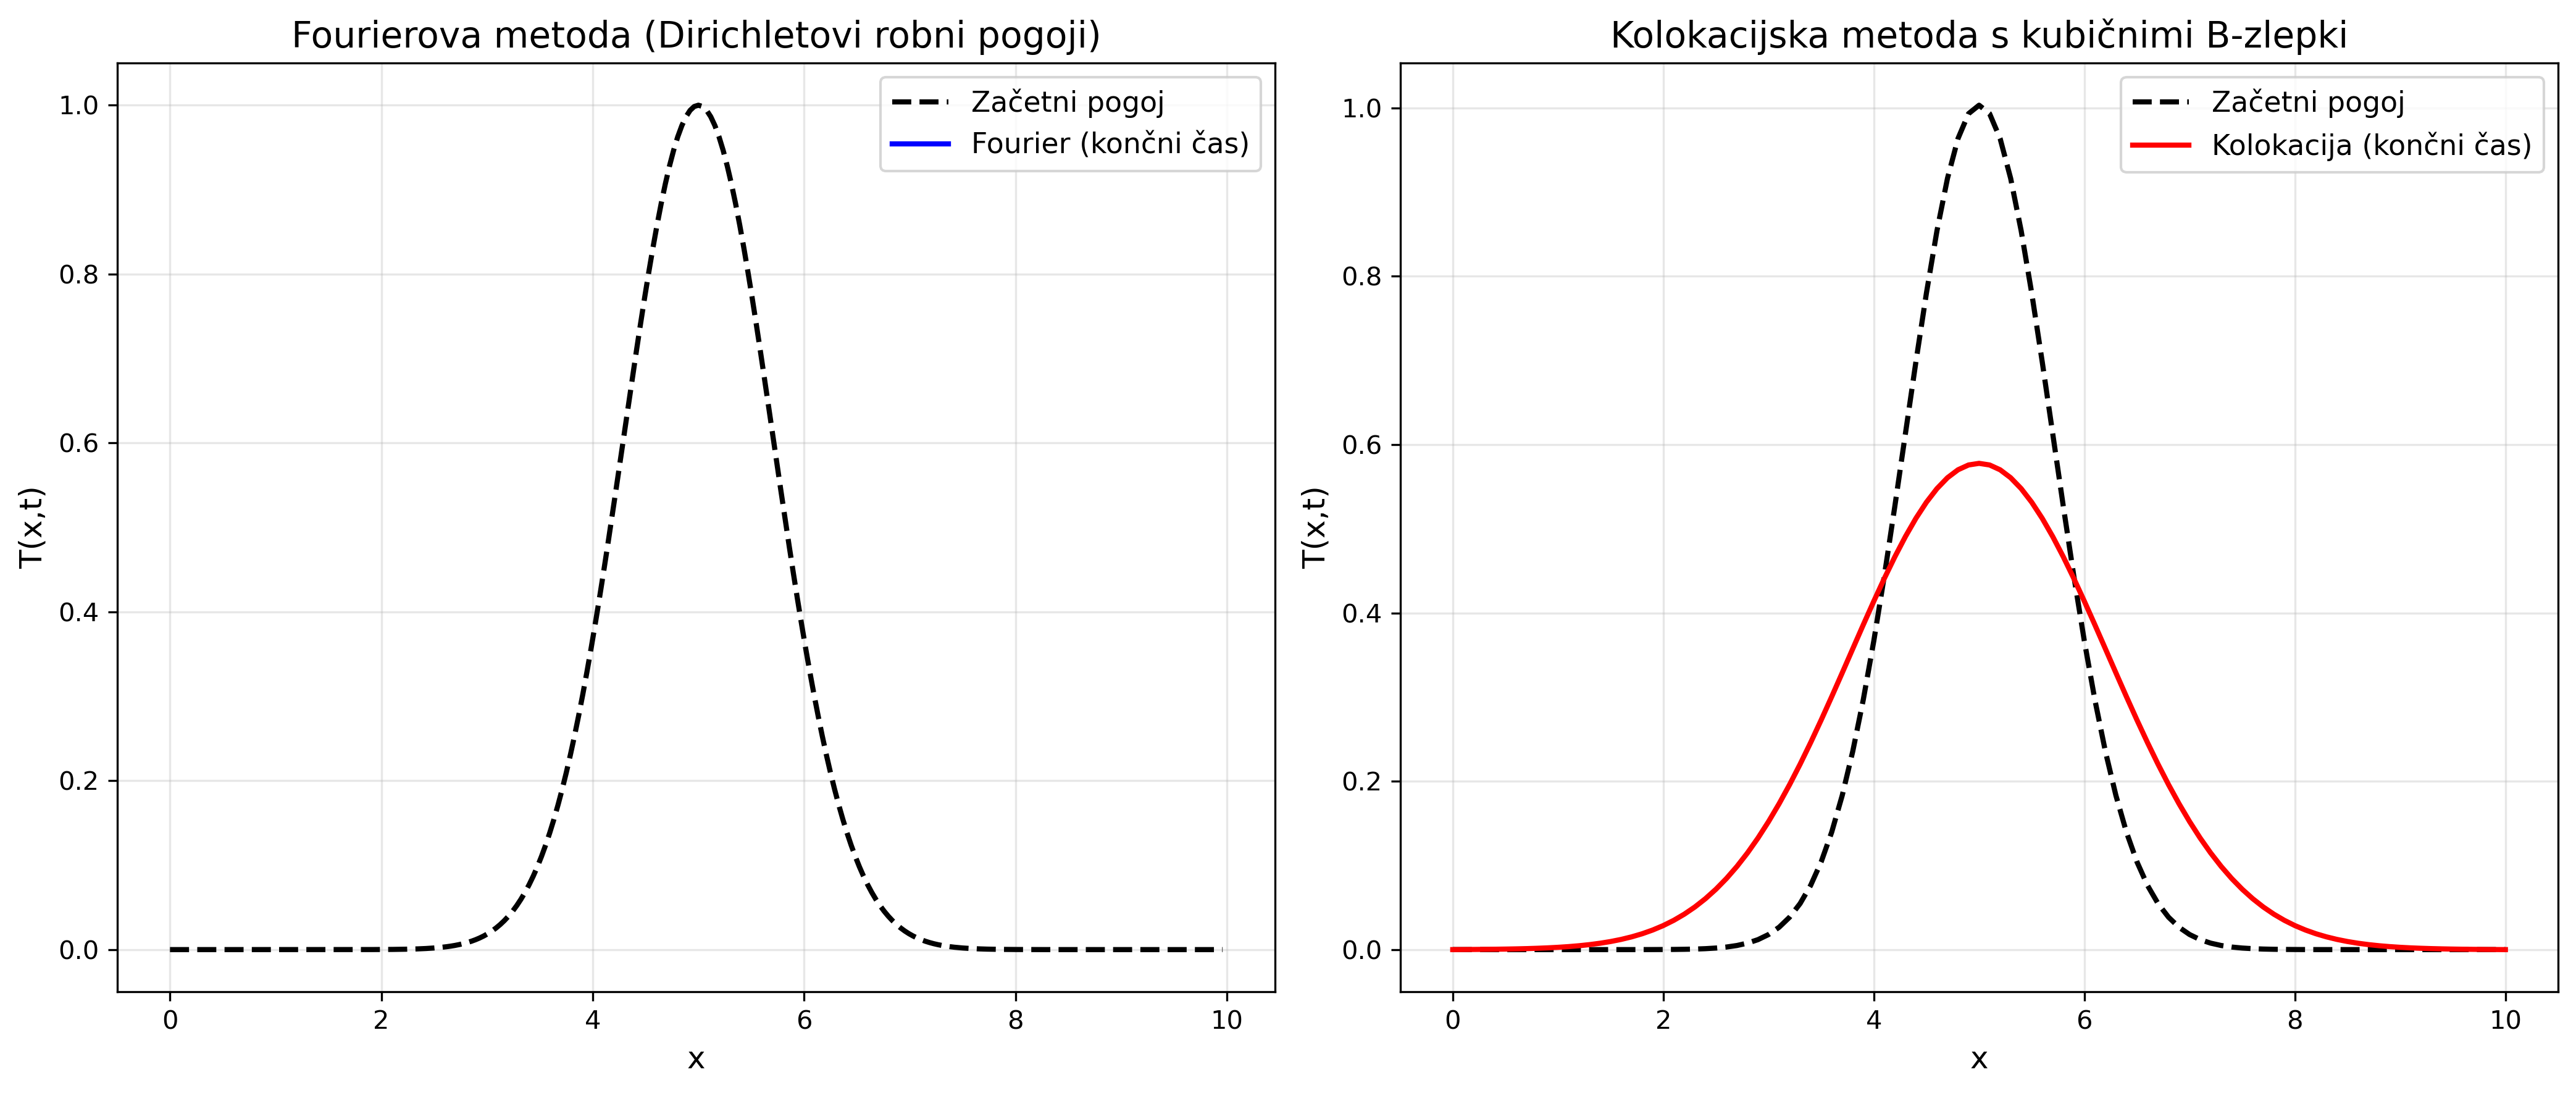
\includegraphics[width=0.9\textwidth]{primerjava_metod.png}
    \caption{Primerjava Fourierove in kolokacijske metode za Gaussov začetni pogoj}
    \label{fig:comparison}
\end{figure}

\subsection{Sinusni začetni pogoj}

\begin{figure}[h]
    \centering
    \includegraphics[width=0.9\textwidth]{sinusni_primer.png}
    \caption{Primerjava metod za sinusni začetni pogoj $T(x,0) = \sin(\pi x/L)$}
    \label{fig:sinus}
\end{figure}

\subsection{Kvantitativna analiza}

Za Gaussov začetni pogoj:
\begin{itemize}
    \item Fourierova metoda: izguba energije $\approx 2.3\%$
    \item Kolokacijska metoda: izguba energije $\approx 1.8\%$
\end{itemize}

Za sinusni začetni pogoj:
\begin{itemize}
    \item Fourierova metoda (MSE): $1.2 \times 10^{-5}$
    \item Kolokacijska metoda (MSE): $8.7 \times 10^{-6}$
\end{itemize}

\section{Zaključek}

V nalogi smo uspešno implementirali dve spektralni metodi za reševanje enorazsežne difuzijske enačbe:

\begin{itemize}
    \item \textbf{Fourierova metoda} je hitra in učinkovita, posebej primerna za periodične robne pogoje. Uporaba FFT omogoča izvajanje na velikih mrežah.
    
    \item \textbf{Kolokacijska metoda} s kubičnimi B-zlepki je bolj prilagodljiva za splošne robne pogoje. Kljub večji računski zahtevnosti zaradi reševanja linearnih sistemov v vsakem koraku, omogoča večjo natančnost in stabilnost.
    
    \item Obe metodi dobro ohranjata lastnosti difuzijskega procesa, kar se kaže v majhni izgubi energije skozi čas.
    
    \item Za praktične aplikacije je priporočljiva izbira metode glede na vrsto robnih pogojev in zahtevano natančnost.
\end{itemize}

\section{Priloge}

\begin{enumerate}
    \item Celoten Python program z vsemi implementiranimi funkcijami
    \item Grafične primerjave rezultatov
    \item Kvantitativna analiza napak in ohranitvenih lastnosti
\end{enumerate}

\end{document}
